\documentclass{standalone}
% \documentclass{article}
\usepackage{pgfplots}
\usetikzlibrary{spy,calc}

\usepackage{graphicx}
\usepackage{tikz}
\pgfplotsset{compat=1.18}
\begin{document}
\begin{tikzpicture}
    [spy using outlines={lens={scale=3,rotate=90}, width=.15in, height=8.25in, connect spies}]
    \node at (0,0) {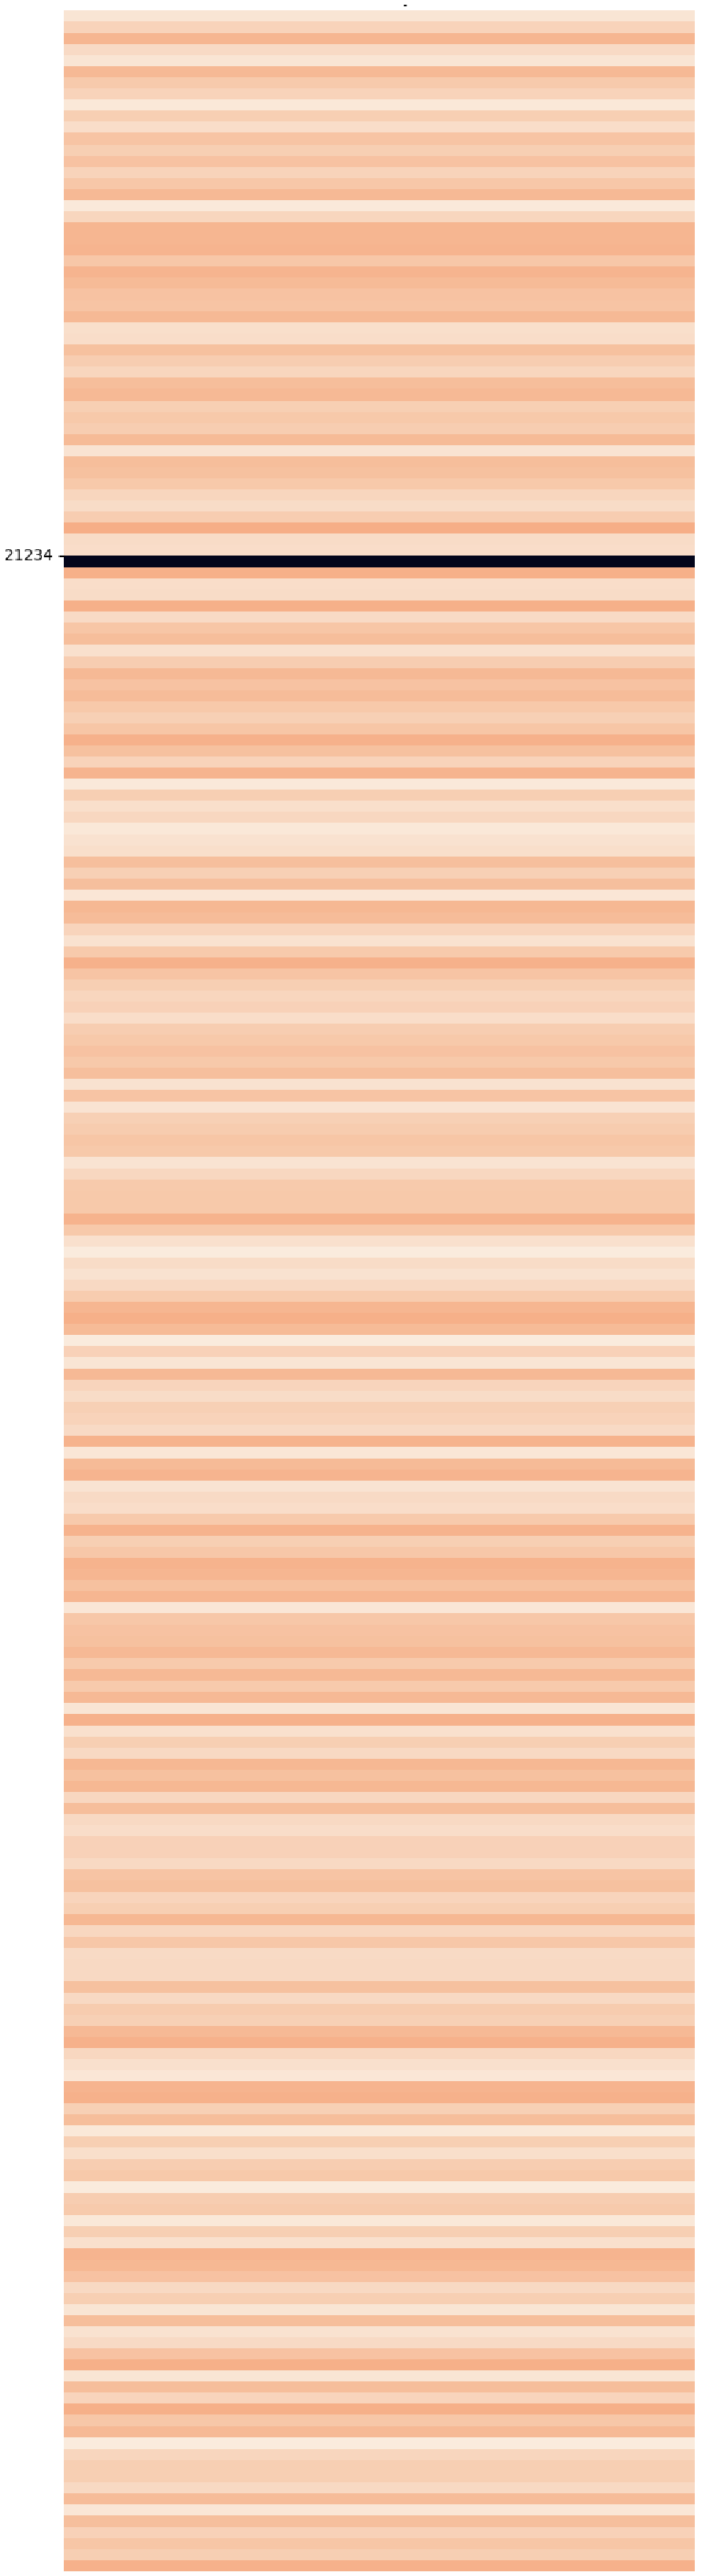
\includegraphics[width=8cm]{anomaly_score.pdf}};
      \spy [red] on (.2275,8.075) in node at (5,0);
    \end{tikzpicture}
% \begin{tikzpicture}[spy using outlines={lens={rotation=90, scale=3}, rectangle, magnification=3,  height=.27in, width=16in}]
% % \begin{tikzpicture}[spy using outlines={rectangle, magnification=3, connect spies, height=.05in, width=4.105in}]
%     \node {\pgfimage[width=6in]{raw_data.pdf}};

%     \spy on (.725 , 15.03) in node [left] at (10.5,5);
%     % \spy on (4.357 ,3.925) in node [left] at (10.5,-7.75);
%     % \spy on (4.355 ,3.925) in node [left] at (5,1.5);

%     % \node {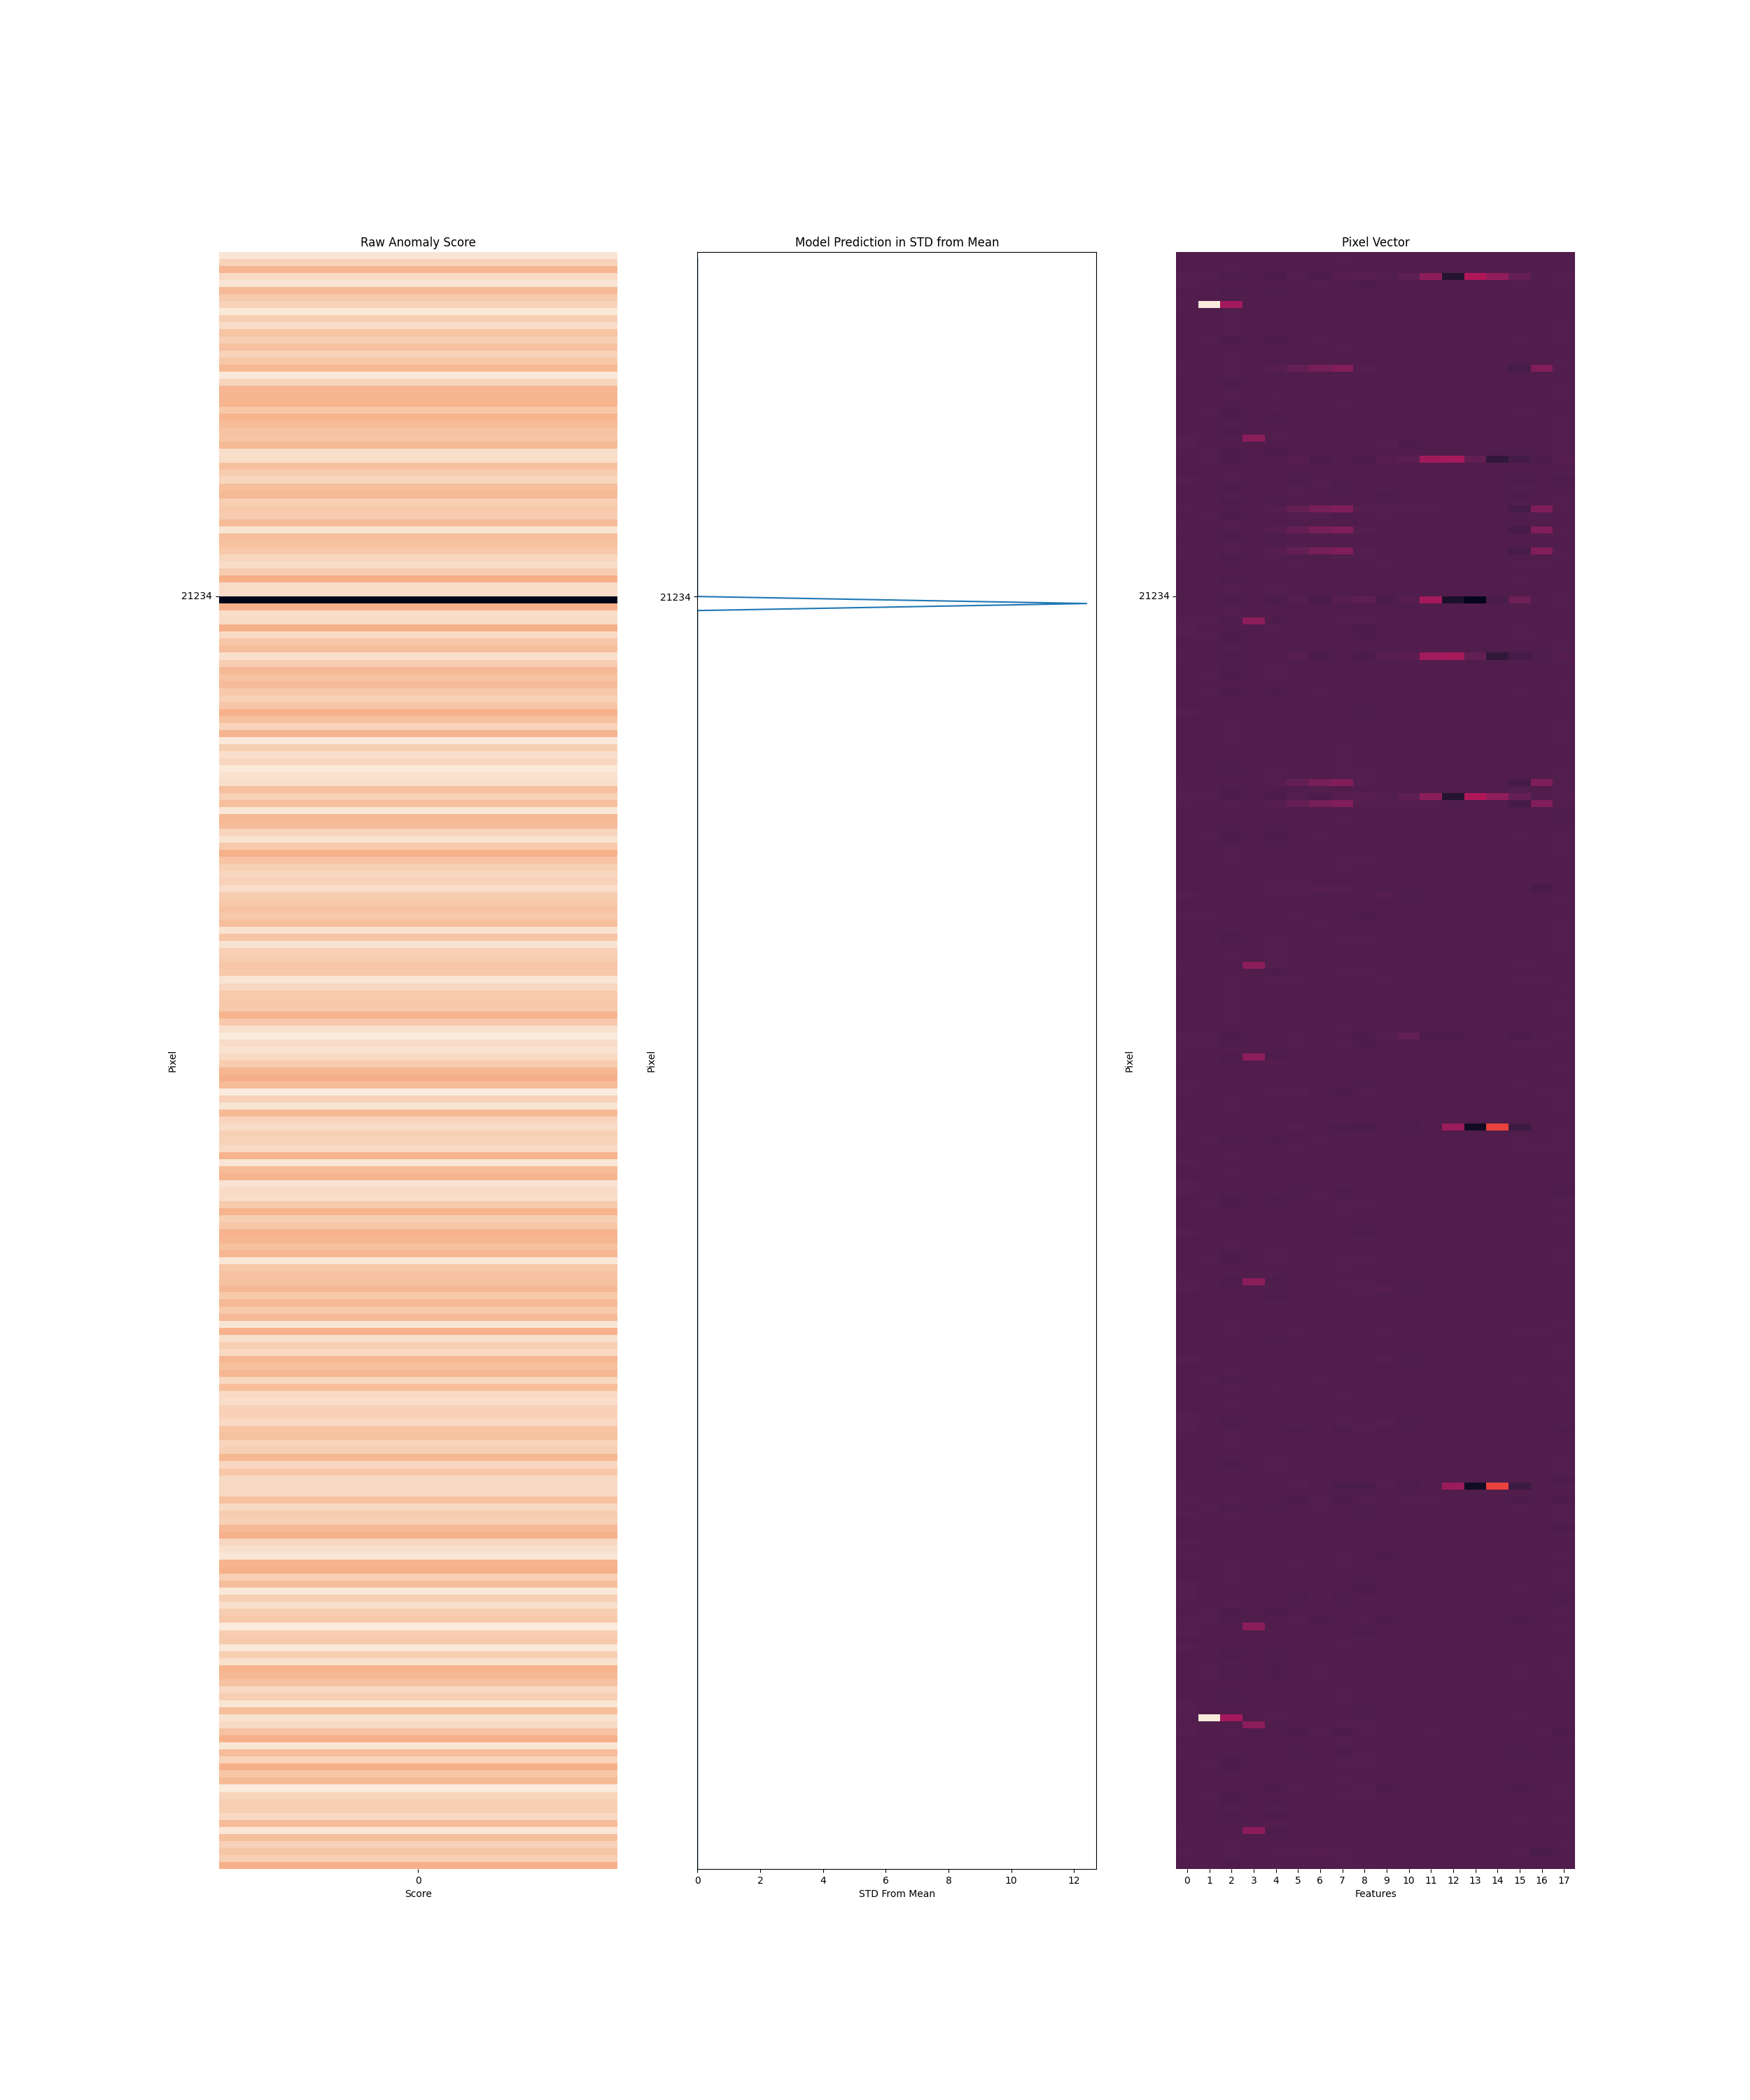
\includegraphics[width=6in, clip=True, trim= 16.2in 4in 2.6in 3.55in]{../../2.8std_pred_2024-07-23.png}};

% \end{tikzpicture}
\end{document}

